%
% Assignment @ DIPT
%
\documentclass[12pt,a4paper]{article}
%
% Set a flag to include or exclude the blue comment boxes.
\usepackage{etoolbox}
\newtoggle{todos}
\toggletrue{todos}
%\togglefalse{todos}
%
% Do only change the row below when changing the template.
% The current date is inserted automatically by command `\date{\today}' below.
\newcommand{\templateVersion}{1.4 -- March 12, 2020}
%
\usepackage[top=2.5cm, bottom=2.5cm, left=2.5cm, right=2.5cm]{geometry} % Sets the size of the document margins
\usepackage[utf8]{inputenc}  % For handling input of special character
\usepackage[T1]{fontenc}  % For better encoding of special characters
%\usepackage[swedish]{babel}  % Uncomment for documents in Swedish
\usepackage{microtype}  % For improved typesetting
\usepackage[hyphens]{url}  % Improved hyphenation of URLs
\usepackage{hyperref}  % For clickable cross-references in the text
\DeclareUrlCommand\email{}  % Formatting of (clickable) email-addresses
\usepackage{enumitem}  % More formatting options for lists
\setlist{topsep=1ex,itemsep=0.5ex,parsep=0pt,partopsep=0pt}  % this sets the vertical spacing between list items and surrounding paragraphs
\usepackage[sort&compress]{natbib}  % Improved formatting of citations
\setcitestyle{numbers,square,comma}
\setlength{\bibsep}{5pt}  % Sets space between two elements in the list of references
\usepackage{multirow}  % Required for table cells that span several rows
\usepackage{longtable}  % Necessary for tables that should span several pages
\usepackage{booktabs}  % Addtl. formatting options for tables
%
\usepackage{listings}  % For pretty printing of source code
%
\iftoggle{todos}{%
  % include the blue comment boxes
  \usepackage[color=blue!10,textsize=footnotesize,textwidth=25mm]{todonotes}
}{%
  % exclude the blue comment boxes
  \usepackage[disable]{todonotes}
}  % Contains commands that we pushed to a separate file.

% Please identify COURSE CODE and COURSE NAME.
\newcommand{\theCourse}{PA1234: Course name}

% Please identify ASSIGNMENT NAME.
\newcommand{\theAssignment}{Assignment name, number and/or title}

% *** Do not touch the following lines. BEGIN. ***
\title{\theAssignment\\\vspace{1mm}\footnotesize{Template version \templateVersion}}
\author{\textsc{\theCourse}}
\date{\today}
%
\begin{document}
%
\maketitle
%
\vspace*{-12mm}
% *** END. Do not touch the lines above. ***

% *** BELOW YOU INSERT BASIC INFORMATION ABOUT THE ASSIGNMENT ***
\begin{longtable}{|l|p{12.15cm}|}
\hline
Group name/ID & Group name or ID, in case this is a group exercise \\ 
\hline
Title         & Title of the answer/ solution \\
\hline
Supervisor(s) & Supervisor name(s), if applicable \\
\hline
\end{longtable}


% *** BELOW YOU INSERT DETAILS ABOUT WHO DID WHAT ***
\vspace*{-7mm}
\begin{small}
\begin{longtable}{|l|l|p{10.9cm}|}
\hline
\multirow{4}{*}{Student 1}
 & Name           & Full name as given in Ladok \\ \cline{2-3}
 & E-Mail         & ...@student.bth.se \\ \cline{2-3}
 & Program        & Program you are registered in \\ \cline{2-3}
 & Contribution   & Contribution of student 1 to this assignment (if there are several students) \\
\hline
\multirow{4}{*}{Student 2}
 & Name           &  \\ \cline{2-3}
 & E-Mail         &  \\ \cline{2-3}
 & Program        &  \\ \cline{2-3}
 & Contribution   &  \\
\hline
\end{longtable}
\end{small}

\todo[inline]{Please add/delete table rows, if necessary. You can leave the rows for group name/ID and/or supervisors empty or delete them, if there are no groups or specific supervisors for the assignment. Don't forget to delete the blue comment-boxes before submission by uncommenting the row \texttt{\textbackslash togglefalse\{todos\}} at the top of the \LaTeX\ source code.}
\todo[inline]{If you use some other text processing software (e.g., Word), please make sure to follow the formatting used in this document as closely as possible.}

% *** BELOW YOU MAINTAIN THE DOCUMENT HISTORY ***
\begin{small}
\begin{longtable}{|l|p{13.3cm}|}
\hline
\multicolumn{2}{|l|}{\textbf{Submission/change history (latest entry on top)}} \\
\textbf{Date} & \textbf{Changes made} \\
\hline
2019-04-01 & Complemented due to FX. Changes made: ... \\
\hline 
2019-03-22 & Initial submission. \\
\hline 
\end{longtable}
\end{small}
\todo[inline]{In the table above, you should briefly describe the revision history of your submission.}

\setcounter{table}{0}  % The tables on the front page shouldn't be counted

% When you need a table of contents, you can uncomment the following line(s)
% \setcounter{tocdepth}{2}  % Sets the level of sections/subsections for the table of contents
% \tableofcontents

\newpage

% *** THE ACTUAL ASSIGNMENT CONTENT STARTS HERE ***
\section{Introduction to the template}
\label{sec:intro}
This document describes in generic terms how a typical assignment submission should look like with respect to formatting and contents.
There are many types and purposes of assignments.
This document can therefore only cover general rules and guidelines.
Please make sure to carefully read the assignment description for your particular assignment, since it might describe additional or more specific requirements.


\section{Sections and subsections}
\label{sec:main}
All assignment submissions should have a Section \textit{Introduction} where you describe the overall purpose of the assignment, introduce key concepts or terms and give a very brief overview over your approach or solution. The remainder of your submission should be structured into sections and subsections that are appropriate for the current assignment. The structure should provide a good high-level overview over your submission, so that it is easy to navigate through the contents and find specific parts. A single \textit{Main}-section will be insufficient, except for very short assignments.
Which sections and/or subsections are required or suitable will differ from assignment to assignment. Examples of sections or subsections for assignments are Prerequisites, Assumptions, Related work, Results, Analysis, Design, Implementation, Limitations, Evaluation, Discussion, Summary, and Conclusions.

The formatting of sections and subsections is exemplified below. Please note that regular paragraphs in sections, subsections, and sub-subsections are not indented. Paragraphs start at the left margin of the page and are aligned left and right, i.e. as in the paragraphs in this document. There is no space between paragraphs. However, the first line of a paragraph is indented, except for the first paragraph in each section, subsection, and sub-subsection.


\subsection{Example subsection header}

\subsubsection{Example sub-subsection header}
Normally, you should not use subsections on levels deeper than three. If you need more structure below level three or if you want to structure your text without numbered headers, you can for example use lists or named paragraphs. You can have bullet-lists, numbered lists, etc. Some examples are shown below. After the example lists, you can also see an example of a named paragraph. 
\begin{itemize}
    \item A list item.
    \item Another list item.
    \begin{enumerate}
        \item Lists can be nested. The text for a single list item may span several lines and should be indented as shown in this example.
        \begin{enumerate}
            \item You should not nest them too deeply, though.
            \item There are more types of lists, but the ones here should do for a start.
        \end{enumerate}
        \item You can also change the numbering scheme, but the standard settings shown here should do for a start. 
    \end{enumerate}
\end{itemize}

\paragraph{Named paragraph.}
Note that named paragraphs are not numbered.


\section{Tables, figures and references}
\label{sec:tab}
In your assignments, you can use tables, figures and references. The entries in the reference list should be sorted alphabetically. Examples of tables and figures are shown below. Their numbering is automatic. Please note that table captions are on top of the tables, whereas figure captions are below the figures.
Please do also note that figures and tables are placed automatically and do not always end up where intended.

\begin{table}[bth]
\centering
\caption{An example of a table.}
\label{tab:ex}
%\begin{small}
\begin{tabular}{|l|r|p{6cm}|}
\hline
\textbf{Items} & \textbf{Number} & \textbf{Comment} \\
\hline
Books & 25 & We categorized everything longer than 50 pages as a book. \\
\hline
Reports & 8 & Blablabla... \\ 
\hline
Etc. & & \\
\hline 
\end{tabular}
%\end{small}
\end{table}

Creating tables and figures can be difficult, since \LaTeX\ is no ``what you see is what you get'' environment. For simple tables, you can use generators, like the one on \url{https://www.tablesgenerator.com} for help. For figures, it is easiest to provide them in separate files and import them using \LaTeX's \texttt{\textbackslash includegraphics} command. The included files can have various formats, like, for example, JPG or PDF.
Using command \texttt{\textbackslash ref}, you can insert cross-references to other places in your document, for example sections (e.g., Section \ref{sec:intro}), tables (e.g., Table \ref{tab:ex}), figures (e.g., Figure \ref{fig:bth}), listings (e.g., Listing \ref{lst:add})), equations (e.g., Equation \ref{eq:fx}), etc. Note that you can only reference places that have a corresponding \texttt{\textbackslash ref} command in the \LaTeX\ code. This command you need to place there manually. For references to literature (citations), there is a special command (\texttt{\textbackslash cite}). You can find examples for that in the next section.

\begin{figure}[bth]
\centering
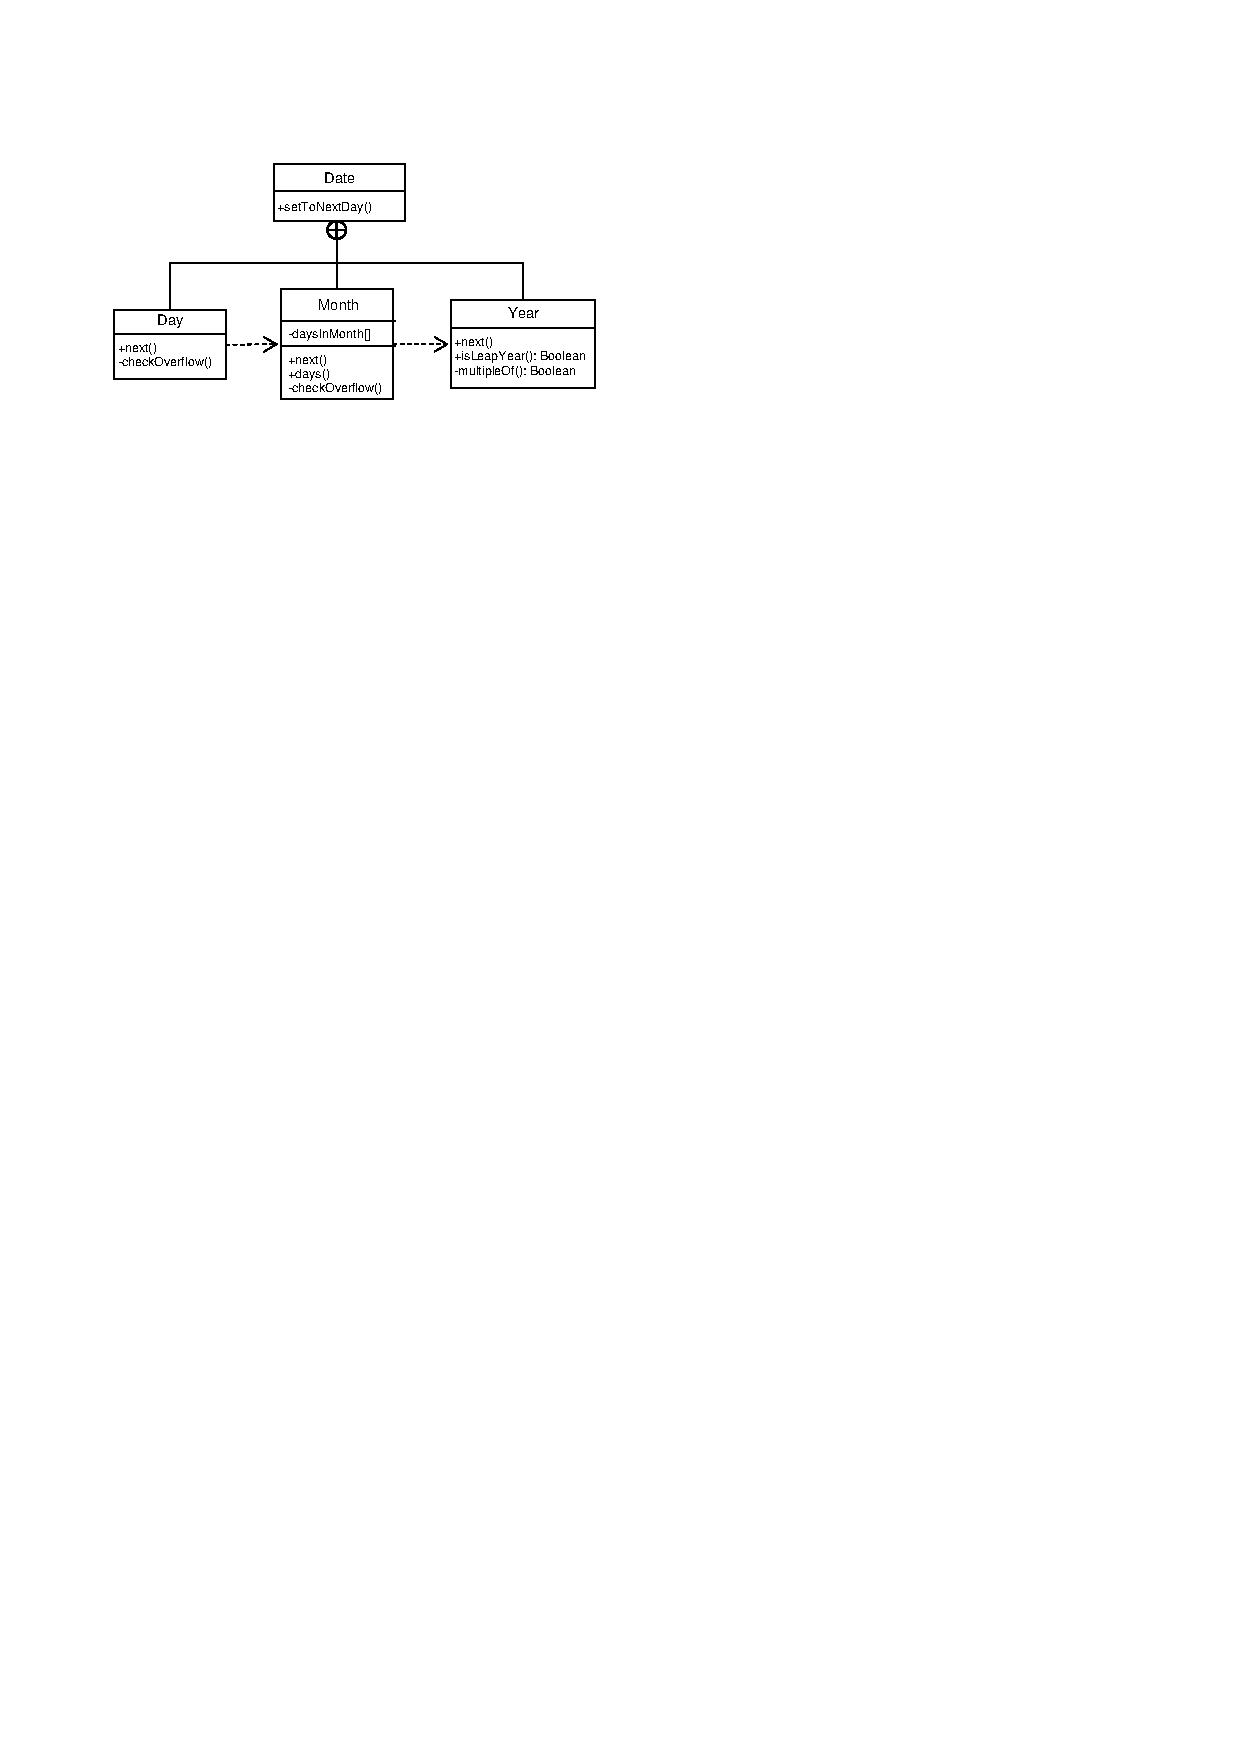
\includegraphics[width=0.6\columnwidth]{example-graph}
\caption{An example graph.}
\label{fig:uml}
\end{figure}

\begin{figure}[bth]
\centering
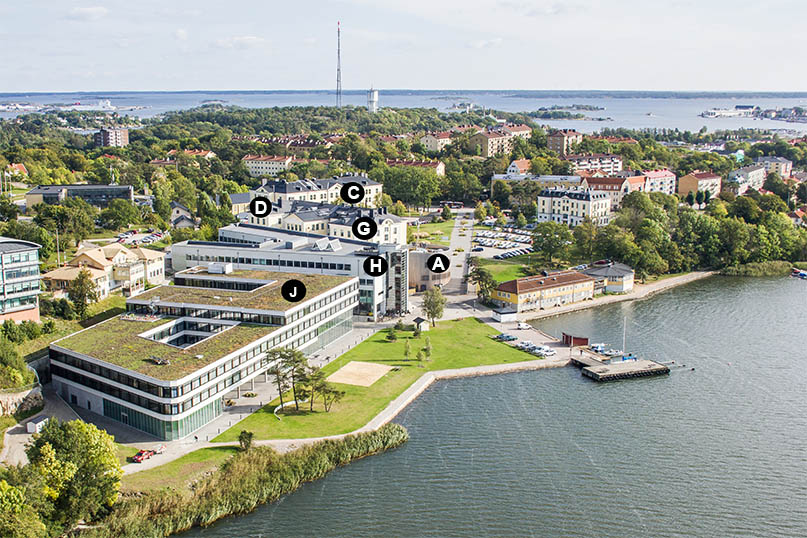
\includegraphics[width=0.6\columnwidth]{example-fig}
\caption{An example figure.}
\label{fig:bth}
\end{figure}


\section{Source code and equations}
\label{sec:code}
Source code can be printed nicely using the \texttt{lstlisting}-environment, as in the example below. There are many parameters for the listings and code can also be loaded from a file. Please check the documentation of package \texttt{listings} for details.

\noindent
\begin{minipage}{\textwidth}
\begin{lstlisting}[frame=single,language=Python,basicstyle=\small,caption={Example of a code-listing.},label={lst:hello}]
# Python3 example for printing a constant string 
print("Hello World!"!)
\end{lstlisting}
\end{minipage}

\lstinputlisting[frame=single,language=Python,basicstyle=\small,caption={Another example of a code-listing.},label={lst:add}]{exampleCode.py}

Equations can be typeset and numbered using the \texttt{equation}-environment, as in equation \ref{eq:fx} below.

\begin{equation}
\label{eq:fx}
    f(x) = (\frac{1}{\sqrt{x}})^2
\end{equation}


\section{More information}
\label{sec:more}
For more details on report writing, please refer to \textit{Rapportskrivning för ingenjörer} \cite{nilsson2018rapport} (Swedish only), which can be downloaded from the library's Writing Guide (Skrivguiden)\footnote{\url{http://skrivguiden.se/resurser/bth-resurser/} (Swedish) or \url{http://writingguide.se/resources/bth-resources/} (English)}.  There are also of resources for learning \LaTeX\ on \url{https://www.overleaf.com/learn}. There are also numerous free guides for learning \LaTeX\ on the Internet (e.g., \cite{oetiker2011not}).

% All references are stored in a separate bib-file: ass-refs.bib
%\clearpage
\small
\bibliographystyle{IEEEtranS}
\bibliography{ass-refs}

\end{document}
